%
% slides.tex
%
% (c) 2019 Prof Dr Andreas Müller, Hochschule Rapperswil
%

\ifthenelse{\boolean{presentation}}{
\begin{frame}
\titlepage
\end{frame}
}{}

\begin{frame}
\frametitle{Skalierungsrelation}
\begin{block}{Aus Multiskalen-Analyse}
Koeffizienten $h_k$ und $g_k$ derart, dass
\begin{align*}
\varphi
&=
\sum_{k\in\mathbb Z}
h_k
D_{\frac12}T_k \varphi
&&\Rightarrow&
\varphi_{j,l} &= \sum_{k\in\mathbb Z} h_k\varphi_{j+1,l+k}
\\
\psi
&=
\sum_{k\in\mathbb Z}
g_k
D_{\frac12}T_k \varphi
&&\Rightarrow&
\psi_{j,l} &= \sum_{k\in\mathbb Z} g_k\varphi_{j+1,l+k}
\end{align*}
\end{block}
\begin{block}{Gesucht: Wavelet-Analyse}
Wavelet-Koeffizienten:
\begin{align*}
a_{j,k} & = \langle f, \varphi_{j,k} \rangle
&&
\\
b_{j,k} & = \langle f, \psi_{j,k} \rangle
&&
\text{Features der Grösse $2^{-j}$ bei $k2^{-j}$}
\end{align*}
\end{block}
\end{frame}

%
% Sampling
%
\begin{frame}
\frametitle{Sampling}
\[
\left.
\begin{aligned}
&\text{$j$ sehr gross}\\
&\uncover<2->{\text{$a_{j,k}=\mathstrut$ Features der Grösse $2^{-j}$}}\\
&\uncover<3->{\text{$f$ ändert nahe bei $k2^{-j}$ langsam}}
\end{aligned}
\uncover<4->{
\quad\right\}
\quad\Rightarrow\quad
\text{$a_{j,k}=\mathstrut$ Funktionswert bei $k2^{-j}$}}
\]
\uncover<5->{
\[
a_{j,k} = \text{Samples mit Auflösung $2^{-j}$}
\]
}
\end{frame}

%
% analyse.tex
%
% (c) 2019 Prof Dr Andreas Müller, Hochschule Rapperswil
%
\section{Analyse}

\begin{frame}
\frametitle{Analyse-Algorithmus}
\begin{align*}
a_{j,k} 
=
\langle f,\varphi_{j,k} \rangle
&\uncover<2->{=
\biggl\langle
f,\sum_{l\in\mathbb Z} h_l\varphi_{j+1,k+l}
\biggr\rangle}
\uncover<3->{=
\sum_{l\in\mathbb Z} \bar{h}_l\langle f, \varphi_{j+1,k+l}\rangle}
\uncover<4->{=
\sum_{l\in\mathbb Z} \bar{h}_la_{j,k+l}}
\\
b_{j,k} 
=
\langle f,\psi_{j,k} \rangle
&\uncover<5->{=
\biggl\langle
f,\sum_{l\in\mathbb Z} g_l\psi_{j+1,k+l}
\biggr\rangle}
\uncover<6->{=
\sum_{l\in\mathbb Z} \bar{g}_l\langle f, \psi_{j+1,k+l}\rangle}
\uncover<7->{=
\sum_{l\in\mathbb Z} \bar{g}_l a_{j+1,k+l}}
\end{align*}
\uncover<8->{
Zweckmässige Reihenfolge der Basisvektoren in $V_j$:
\[
\dots,
\varphi_{j,-2},
\psi_{j,-2},
\varphi_{j,-1},
\psi_{j,-1},
\varphi_{j,0},
\psi_{j,0},
\varphi_{j,1},
\psi_{j,1},
\varphi_{j,2},
\psi_{j,2},
\dots
\]
}
\end{frame}

\begin{frame}
\frametitle{Analyse}
Am Beispiel des Haar-Wavelets:
\[
\xymatrix{
a_{j,-2} \ar[d] \ar[dr]
	&a_{j,-1} {\color{red}\ar[d]^{\cdot (-1)}} \ar[dl]
		&a_{j,0} \ar[d] \ar[dr]
			&a_{j,1} {\color{red}\ar[d]^{\cdot (-1)}} \ar[dl]
				&a_{j,2} \ar[d] \ar[dr]
					&a_{j,3} {\color{red}\ar[d]^{\cdot (-1)}} \ar[dl]
						&\dots
\\
a_{j-1,-1} {\color{red}\ar[d]^{\cdot(-1)}}
	&b_{j-1,-1}
		&a_{j-1,0}\ar[d] \ar[drr]
			&b_{j-1,0}
				&a_{j-1,1} {\color{red}\ar[d]^{\cdot (-1)}} \ar[dll]
					&b_{j-1,1}
						&\dots
\\
b_{j-2,-1} 
	&
		&a_{j-2,0} \ar[d] \ar[drrrr]
			&
				&b_{j-2,0}
					&
						&\dots \ar[dllll]
\\
	&
		&a_{j-3,0}
			&
				&
					&
						&\dots
}
\]
\end{frame}

\begin{frame}
\frametitle{Analyse in Matrixform}
\bgroup
\setlength{\tabcolsep}{4pt}
\def\arraystretch{1.3}
\begin{tabular}{>{$}c<{$}|
>{$}c<{$}
>{$}c<{$}
>{$}c<{$}
>{$}c<{$}
>{$}c<{$}
>{$}c<{$}
>{$}c<{$}
>{$}c<{$}
>{$}c<{$}
>{$}c<{$}|}
        &\dots &a_{j+1,-2}  &a_{j+1,-1}  &a_{j+1,0}   &a_{j+1,1}   &a_{j+1,2}   &a_{j+1,3}   &a_{j+1,4}&a_{j+1,5}&\dots \\
\hline
\vdots  &\ddots&\vdots      &\vdots      &\vdots      &\vdots      &\vdots      &\vdots      &\vdots   &\vdots   &\ddots\\
a_{j,-2}&\dots &\bar{h}_2   &\bar{h}_3   &\bar{h}_4   &\bar{h}_5   &\bar{h}_6   &\bar{h}_7   &\bar{h}_8&\bar{h}_9&\dots \\
b_{j,-2}&\dots &\bar{g}_2   &\bar{g}_3   &\bar{g}_4   &\bar{g}_5   &\bar{g}_6   &\bar{g}_7   &\bar{g}_8&\bar{g}_9&\dots \\
a_{j,-1}&\dots &\bar{h}_0   &\bar{h}_1   &\bar{h}_2   &\bar{h}_3   &\bar{h}_4   &\bar{h}_5   &\bar{h}_6&\bar{h}_7&\dots \\
b_{j,-1}&\dots &\bar{g}_0   &\bar{g}_1   &\bar{g}_2   &\bar{g}_3   &\bar{g}_4   &\bar{g}_5   &\bar{g}_6&\bar{g}_7&\dots \\
a_{j, 0}&\dots &\bar{h}_{-2}&\bar{h}_{-1}&\bar{h}_0   &\bar{h}_1   &\bar{h}_2   &\bar{h}_3   &\bar{h}_4&\bar{h}_5&\dots \\
b_{j, 0}&\dots &\bar{g}_{-2}&\bar{g}_{-1}&\bar{g}_0   &\bar{g}_1   &\bar{g}_2   &\bar{g}_3   &\bar{g}_4&\bar{g}_5&\dots \\
a_{j, 1}&\dots &\bar{h}_{-4}&\bar{h}_{-3}&\bar{h}_{-2}&\bar{h}_{-1}&\bar{h}_0   &\bar{h}_1   &\bar{h}_2&\bar{h}_3&\dots \\
b_{j, 1}&\dots &\bar{g}_{-4}&\bar{g}_{-3}&\bar{g}_{-2}&\bar{g}_{-1}&\bar{g}_0   &\bar{g}_1   &\bar{g}_2&\bar{g}_3&\dots \\
a_{j, 2}&\dots &\bar{h}_{-6}&\bar{h}_{-5}&\bar{h}_{-4}&\bar{h}_{-3}&\bar{h}_{-2}&\bar{h}_{-1}&\bar{h}_0&\bar{h}_1&\dots \\
b_{j, 2}&\dots &\bar{g}_{-6}&\bar{g}_{-5}&\bar{g}_{-4}&\bar{g}_{-3}&\bar{g}_{-2}&\bar{g}_{-1}&\bar{g}_0&\bar{g}_1&\dots \\
\vdots  &\ddots&\vdots      &\vdots      &\vdots      &\vdots      &\vdots      &\vdots      &\vdots   &\vdots   &\ddots\\
\hline
\end{tabular}
\egroup
\end{frame}


%
% umkehrung.tex -- Umkehrtransformation
%
% (c) 2019 Prof Dr Andreas Müller
%
\section{Umkehrung}

%
% Basistransformation
%
\begin{frame}
\frametitle{Basistransformation}
\begin{block}{Basen}
Orthonormierte
Basen $\mathcal{B}=\{b_j\,|\,1\le j\le n\}$ und
$\mathcal{C}=\{c_j\,|\,1\le j\le n\}$:
\[
v
=
\sum_i \xi_i b_i
\uncover<2->{=
\sum_l \eta_l c_l}
\]
\end{block}
\uncover<3->{
\begin{block}{Transformationsmatrix}
\[
b_i
=
\sum_{j} t_{ji} c_j
\uncover<4->{
\quad\Rightarrow\quad
v
=
\sum_i\xi_i b_i
}
\uncover<5->{=
\sum_{j,i} t_{ji}\xi_i c_j}
\uncover<6->{\quad\Rightarrow\quad
\eta_j = \sum_i t_ji\xi_i}
\uncover<7->{\quad\Rightarrow\quad
\eta = T\xi}
\]
\end{block}
}
\end{frame}

%
% Orthogonalität
%
\begin{frame}
\frametitle{Orthogonalität}
$b_i$ und $c_j$ sind orthogonal:
\[
\langle b_i,b_j\rangle=\delta_{ij}\;\forall i,j
\qquad\text{und}\qquad
\langle c_i,c_j\rangle=\delta_{ij}\;\forall i,j
\]
\uncover<2->{
\begin{block}{Transformationsmatrix}
\[
\langle b_i,b_j\rangle
\uncover<3->{=
\biggl\langle
\sum_{k} t_{ki} c_k,
\sum_{l} t_{lj} c_l
\biggr\rangle}
\uncover<4->{=
\sum_{k,l}
t_{ki} \bar{t}_{lj}
\underbrace{
\langle c_k, c_l\rangle
}_{\displaystyle=\delta_{kl}}}
\uncover<5->{=
\sum_{k}
t_{ki} \bar{t}_{kj}}
\uncover<6->{=
\sum_{k}
\bar{t}_{kj}
t_{ki}}
\]
\uncover<7->{Notation: $T^* =\overline{T}^t$, komplex konjugierte und transponierte Matrix $T$}
\uncover<8->{%
\[
T^*T = E
\uncover<9->{\quad\Rightarrow\quad
T^{-1} = T^*}
\]
}%
\uncover<10->{``orthogonale komplexe Matrix'', unitäre Matrix}
\end{block}
}
\end{frame}

%
% Umkehrtransformation für die Wavelet-Transformation
%
\begin{frame}
\frametitle{Umkehrtransformation --- Matrixform}
\bgroup
\setlength{\tabcolsep}{4pt}
\def\arraystretch{1.5}
\begin{tabular}{>{$}c<{$}|
>{$}c<{$}
>{$}c<{$}
>{$}c<{$}
>{$}c<{$}
>{$}c<{$}
>{$}c<{$}
>{$}c<{$}
>{$}c<{$}
>{$}c<{$}
>{$}c<{$}
>{$}c<{$}
>{$}c<{$}|}
          &\dots &a_{j,-2}&b_{j,-2}&a_{j,-1}&b_{j,-1}&a_{j,0}&b_{j,0}&a_{j,1}&b_{j,1}&a_{j,2}&b_{j,2}&\dots \\
\hline
\vdots    &\ddots&\vdots  &\vdots  &\vdots  &\vdots  &\vdots &\vdots &\vdots &\vdots &\vdots &\vdots &\ddots\\
a_{j+1,-2}&\dots &h_{ 2}  &g_{ 2}  &h_{ 0}  &g_{ 0}  &h_{-2} &g_{-2} &h_{-4} &g_{-4} &h_{-6} &g_{-6} &\dots \\
a_{j+1,-1}&\dots &h_{ 3}  &g_{ 3}  &h_{ 1}  &g_{ 1}  &h_{-1} &g_{-1} &h_{-3} &g_{-3} &h_{-5} &g_{-5} &\dots \\
a_{j+1, 0}&\dots &h_{ 4}  &g_{ 4}  &h_{ 2}  &g_{ 2}  &h_{ 0} &g_{ 0} &h_{-2} &g_{-2} &h_{-4} &g_{-4} &\dots \\
a_{j+1, 1}&\dots &h_{ 5}  &g_{ 5}  &h_{ 3}  &g_{ 3}  &h_{ 1} &g_{ 1} &h_{-1} &g_{-1} &h_{-3} &g_{-3} &\dots \\
a_{j+1, 2}&\dots &h_{ 6}  &g_{ 6}  &h_{ 4}  &g_{ 4}  &h_{ 2} &g_{ 2} &h_{ 0} &g_{ 0} &h_{-2} &g_{-2} &\dots \\
a_{j+1, 3}&\dots &h_{ 7}  &g_{ 7}  &h_{ 5}  &g_{ 5}  &h_{ 3} &g_{ 3} &h_{ 1} &g_{ 1} &h_{-1} &g_{-1} &\dots \\
a_{j+1, 4}&\dots &h_{ 8}  &g_{ 8}  &h_{ 6}  &g_{ 6}  &h_{ 4} &g_{ 4} &h_{ 2} &g_{ 2} &h_{ 0} &g_{ 0} &\dots \\
a_{j+1, 5}&\dots &h_{ 9}  &g_{ 9}  &h_{ 7}  &g_{ 7}  &h_{ 5} &g_{ 5} &h_{ 3} &g_{ 3} &h_{ 1} &g_{ 1} &\dots \\
\vdots    &\ddots&\vdots  &\vdots  &\vdots  &\vdots  &\vdots &\vdots &\vdots &\vdots &\vdots &\vdots &\ddots\\
\hline
\end{tabular}
\egroup

\end{frame}

\begin{frame}
\frametitle{Umkehrtransformation --- Formel}
Transformationsformeln:
\[
\begin{aligned}
a_{j+1,k}
&=
\dots
+
h_{k+4}
a_{j,-2}
+
g_{k+4}
b_{j,-2}
+
h_{k+2}
a_{j,-1}
+
g_{k+2}
b_{j,-1}
\\
&\qquad
+
h_{k}
a_{j,0}
+
g_{k}
b_{j,0}
+
h_{k-2}
a_{j,1}
+
g_{k-2}
b_{j,1}
+
\dots
\\
&\uncover<2->{=
\dots
+
h_{k+4}
a_{j,-2}
+
h_{k+2}
a_{j,-1}
+
h_{k}
a_{j,0}
+
h_{k-2}
a_{j,1}}
\\
&\uncover<3->{\qquad
+
g_{k+4}
b_{j,-2}
+
g_{k+2}
b_{j,-1}
+
g_{k}
b_{j,0}
+
g_{k-2}
b_{j,1}
+
\dots}
\\
&\uncover<4->{=
\sum_{l\in\mathbb Z}
h_{k-2l}
a_{j,l}
+
\sum_{l\in\mathbb Z}
g_{k-2l}
b_{j,l}.}
\end{aligned}
\]
\end{frame}


%
% db.tex -- Daubechies wavelets als Beispiele
%
% (c) 2019 Prof Dr Andreas Müller, Hochschule Rapperswil
%
\section{Rekonstruktion}

%
% Rekonstruktion
%
\begin{frame}
\frametitle{Rekonstruktion}
\begin{block}{Vater-Wavelet}
Analysiere $f = \varphi_{j,0}$
\[
\left.
\begin{aligned}
\langle\varphi_{j,0},\varphi_{j,k}\rangle&=\delta_{jk}
\\
\langle\varphi_{j,0},\psi_{j,k}\rangle&=0
\end{aligned}
\quad
\right\}
\quad \Rightarrow \quad
\text{Rekonstruieren aus $a_{0,0}=1$}
\]
\end{block}

\begin{block}{Mutter-Wavelet}
Analysiere $f = \psi_{j,0}$
\[
\left.
\begin{aligned}
\langle\psi_{j,0},\varphi_{j,k}\rangle&=0
\\
\langle\psi_{j,0},\psi_{j,k}\rangle&=\delta_{jk}
\end{aligned}
\quad
\right\}
\quad \Rightarrow \quad
\text{Rekonstruieren aus $b_{0,0}=1$}
\]
\end{block}

\end{frame}

%
% Wavelet Koeffizienten für \varphi
%
\begin{frame}
\frametitle{Koeffizienten von $\varphi$ \uncover<4->{und $\psi$}}
\begin{center}
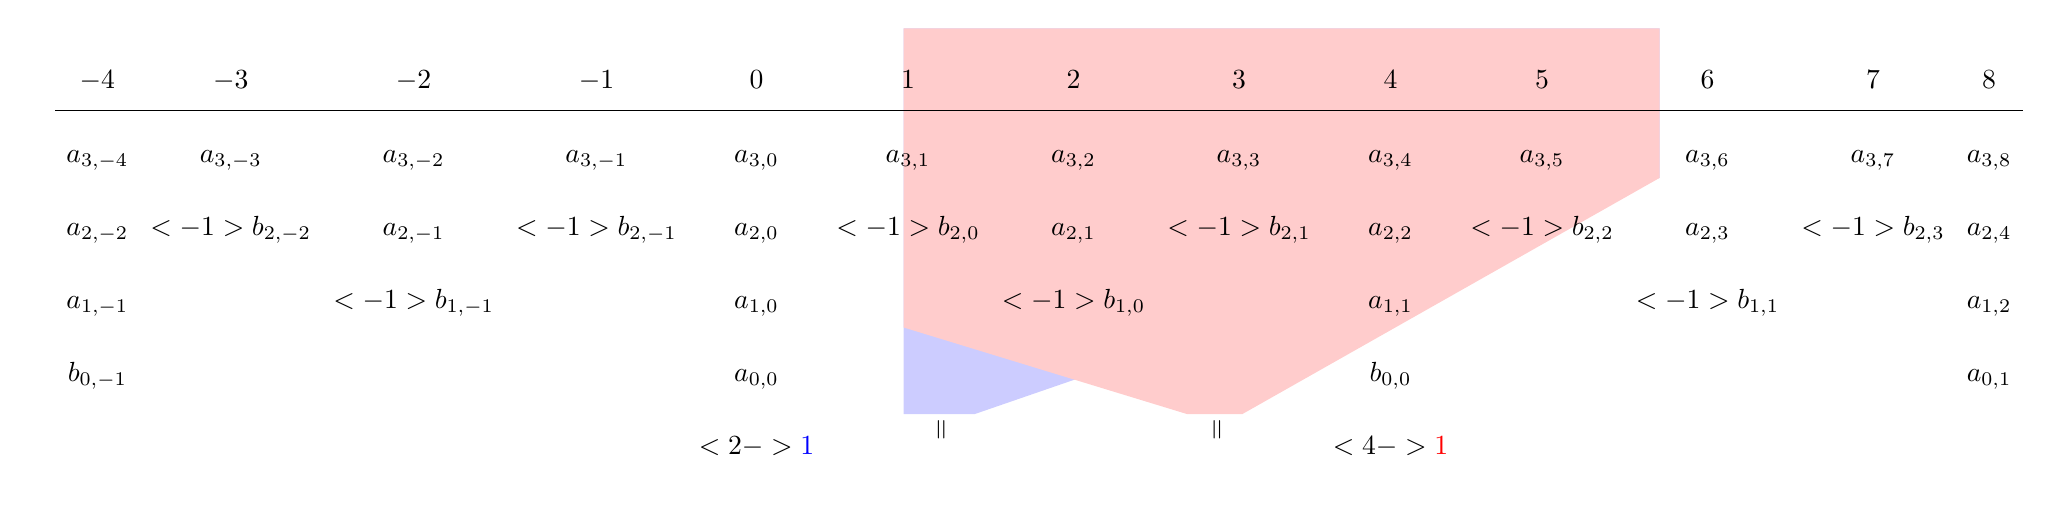
\begin{tikzpicture}[>=latex]
\uncover<3>{
\fill[color=blue!20] (-1.6,2.9)--(-1.6,-2.0)--(-0.7,-2.0)--(8,1)--(8,2.9)--cycle;
}
\uncover<5>{
\fill[color=red!20] (-1.6,2.9)--(-1.6,-0.9)--(2.0,-2.0)--(2.7,-2.0)--(8,1)--(8,2.9)--cycle;

}
\node at (0,0) {
\bgroup
\def\arraystretch{2.2}
\setlength{\tabcolsep}{4pt}
\begin{tabular}{
>{$}c<{$}
>{$}c<{$}
>{$}c<{$}
>{$}c<{$}
>{$}c<{$}
>{$}c<{$}
>{$}c<{$}
>{$}c<{$}
>{$}c<{$}
>{$}c<{$}
>{$}c<{$}
>{$}c<{$}
>{$}c<{$}
}
-4&-3&-2&-1&0&1&2&3&4&5&6&7&8
\\
\hline
a_{3,-4}&a_{3,-3}&a_{3,-2}&a_{3,-1}
&a_{3,0}&a_{3,1}&a_{3,2}&a_{3,3}&a_{3,4}
&a_{3,5}&a_{3,6}&a_{3,7} &a_{3,8}
\\
a_{2,-2}&\uncover<-1>{b_{2,-2}}&a_{2,-1}&\uncover<-1>{b_{2,-1}}
&a_{2,0}&\uncover<-1>{b_{2,0}}&a_{2,1}&\uncover<-1>{b_{2,1}}
&a_{2,2}&\uncover<-1>{b_{2,2}}&a_{2,3}&\uncover<-1>{b_{2,3}}
&a_{2,4}
\\
a_{1,-1}&&\uncover<-1>{b_{1,-1}}&&
a_{1,0}&&\uncover<-1>{b_{1,0}}&&
a_{1,1}&&\uncover<-1>{b_{1,1}}&&
a_{1,2}
\\
b_{0,-1}&&&
&a_{0,0}&&&
&b_{0,0}&&&
&a_{0,1}
\\
&&&
&\uncover<2->{\color{blue}1}&&&
&\uncover<4->{\color{red}1}&&&
&
\end{tabular}
\egroup
};
\uncover<2->{\node at (-1.1,-2.2) [rotate=90] {$=$};}
\uncover<4->{\node at ( 2.4,-2.2) [rotate=90] {$=$};}
\end{tikzpicture}
\end{center}
\end{frame}

%
% db2-Haar-Wavelet
%
\begin{frame}
\frametitle{db2 -- Haar}
\begin{columns}[T]
\begin{column}{2.5cm}
Koeffizienten:
\[
\begin{aligned}
h_0&=\phantom{-}1\\
h_1&=\phantom{-}1\\[10pt]
g_0&=\phantom{-}1\\
g_1&=-1\\
\end{aligned}
\]
\end{column}
\begin{column}{9.5cm}
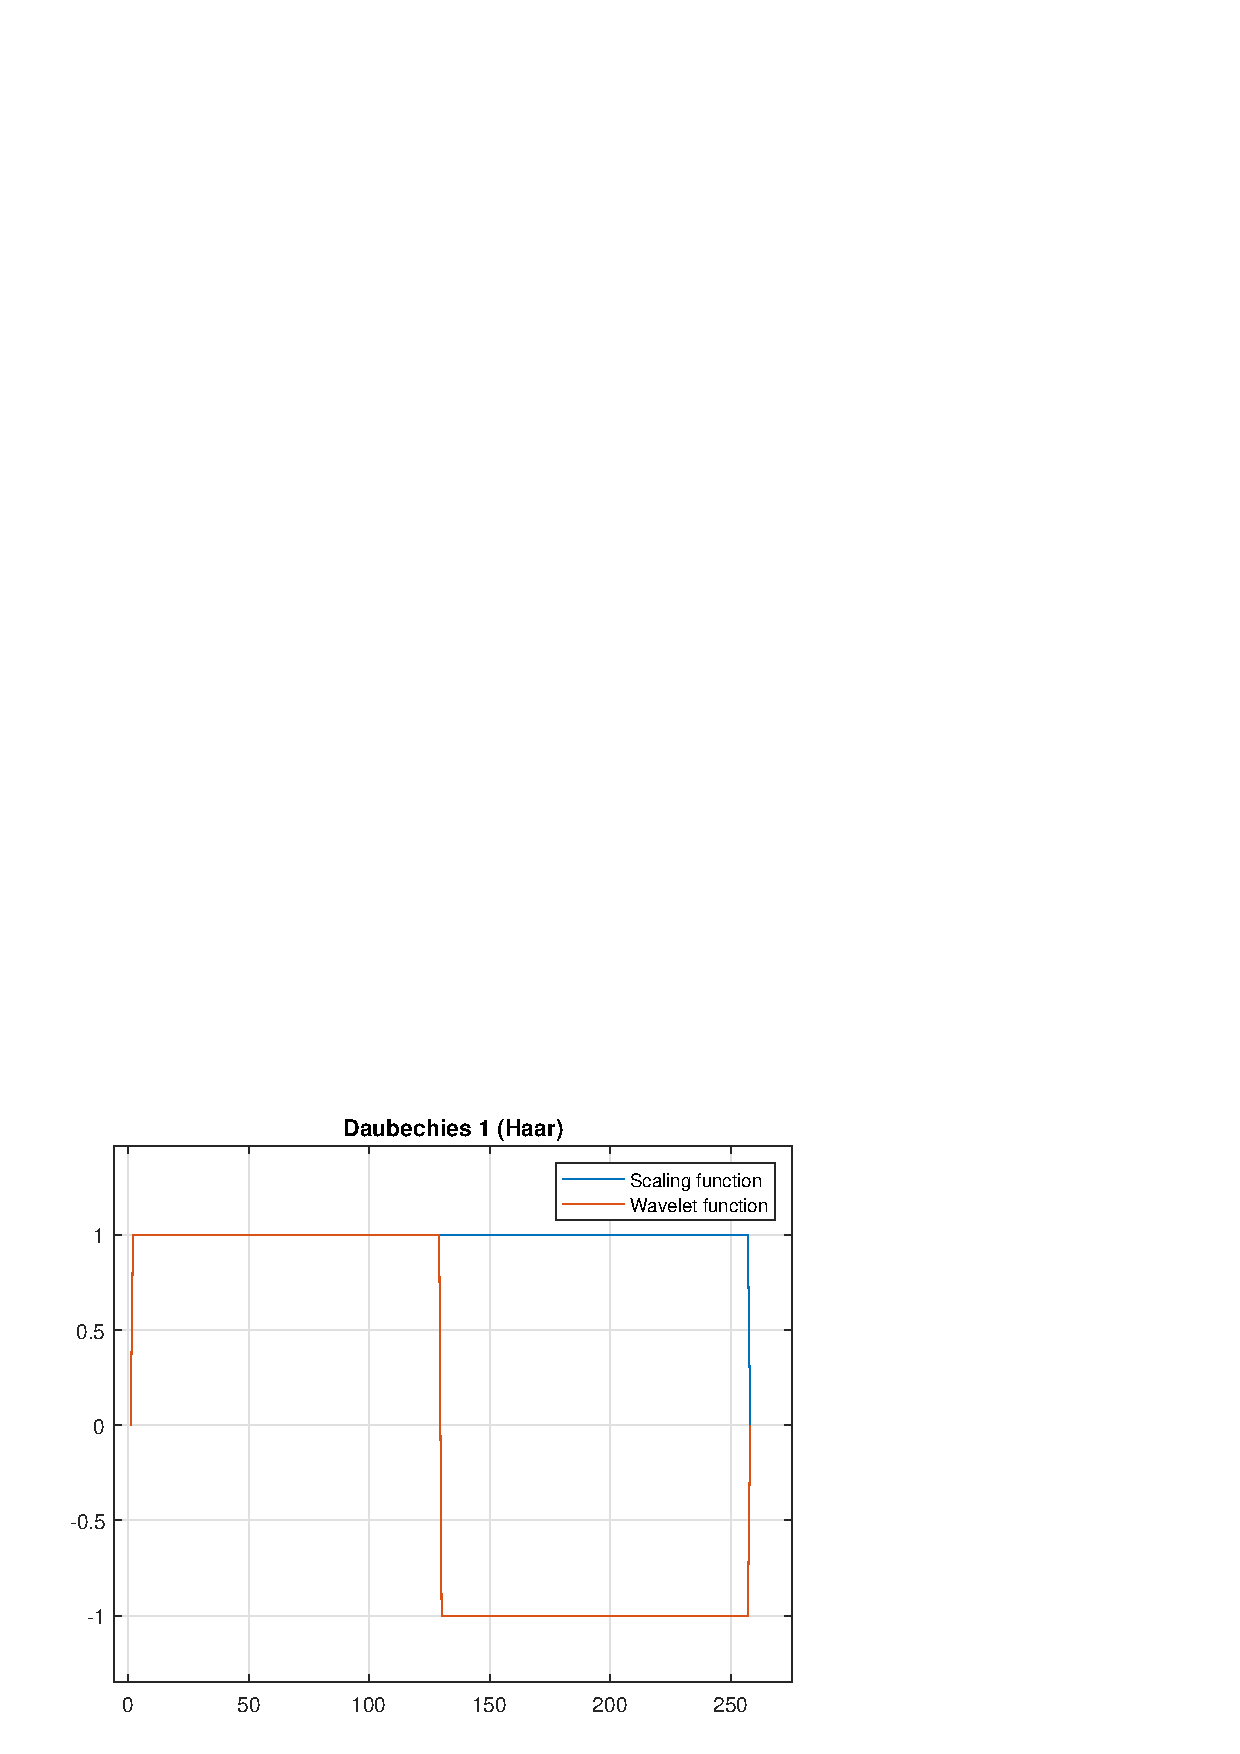
\includegraphics{../../buch/chapters/7-algo/images/db1.pdf}
\end{column}
\end{columns}
\end{frame}


\begin{frame}
\frametitle{db4}
\begin{columns}[T]
\begin{column}{2.5cm}
Koeffizienten:
\[
\begin{aligned}
h_0&=\phantom{-}0.6830127\\
h_0&=\phantom{-}1.1830127\\
h_0&=\phantom{-}0.3169873\\
h_0&=-0.1830127\\[10pt]
g_0&=\phantom{-}0.1830127\\
g_1&=-0.3169873\\
g_2&=\phantom{-}1.1830127\\
g_3&=-0.6830127
\end{aligned}
\]
\end{column}
\begin{column}{9.5cm}
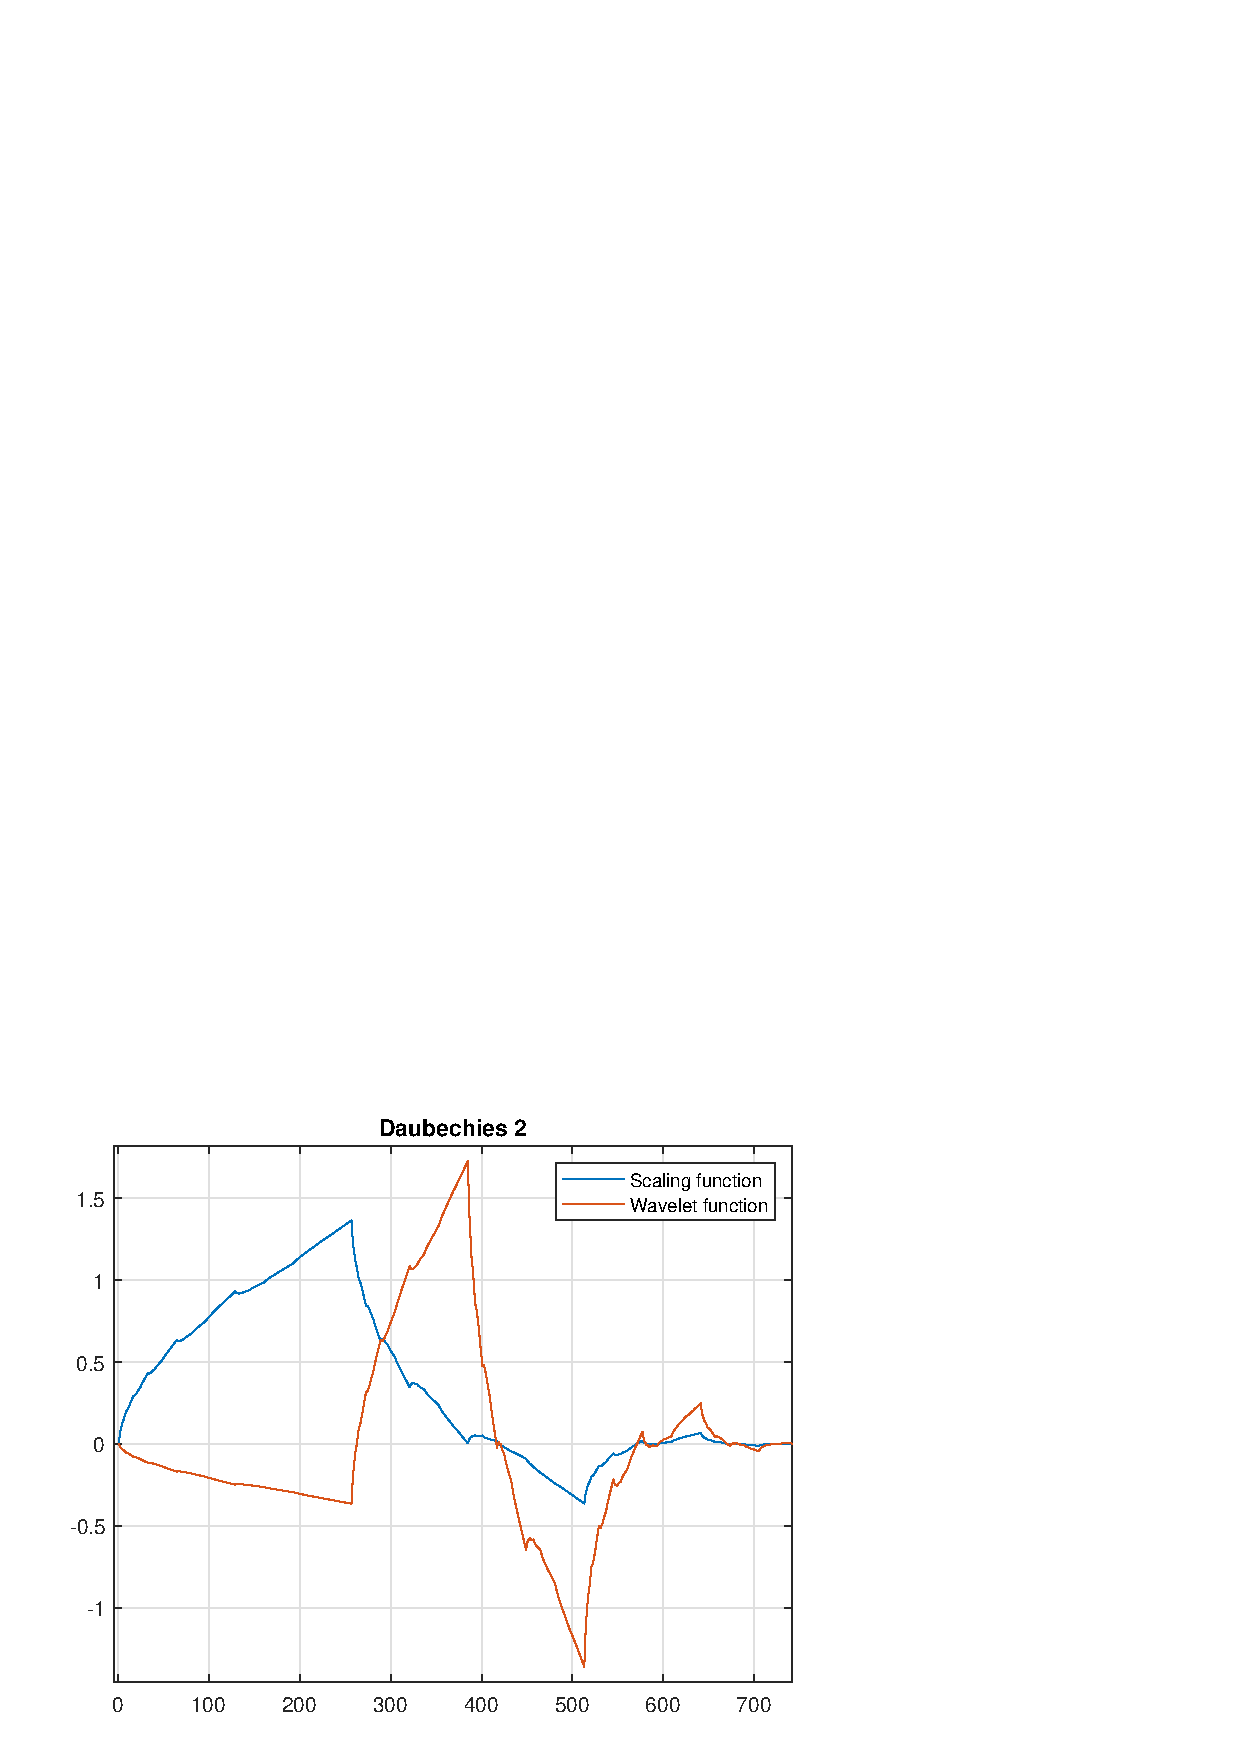
\includegraphics{../../buch/chapters/7-algo/images/db2.pdf}
\end{column}
\end{columns}
\end{frame}

\begin{frame}
\frametitle{db6}
\begin{columns}[T]
\begin{column}{2.5cm}
Koeffizienten:
\[
\begin{aligned}
h_0&=\phantom{-}0.32580343\\
h_0&=\phantom{-}1.01094572\\
h_0&=\phantom{-}0.8922014\\
h_0&=-0.03967503\\
h_0&=-0.26450717\\
h_0&=\phantom{-}0.0436163\\
h_0&=\phantom{-}0.0465036\\
h_0&=-0.01498699
\end{aligned}
\]
\end{column}
\begin{column}{9.5cm}
\includegraphics{../../buch/chapters/7-algo/images/db3.pdf}
\end{column}
\end{columns}
\end{frame}

\begin{frame}
\frametitle{db8}
\begin{center}
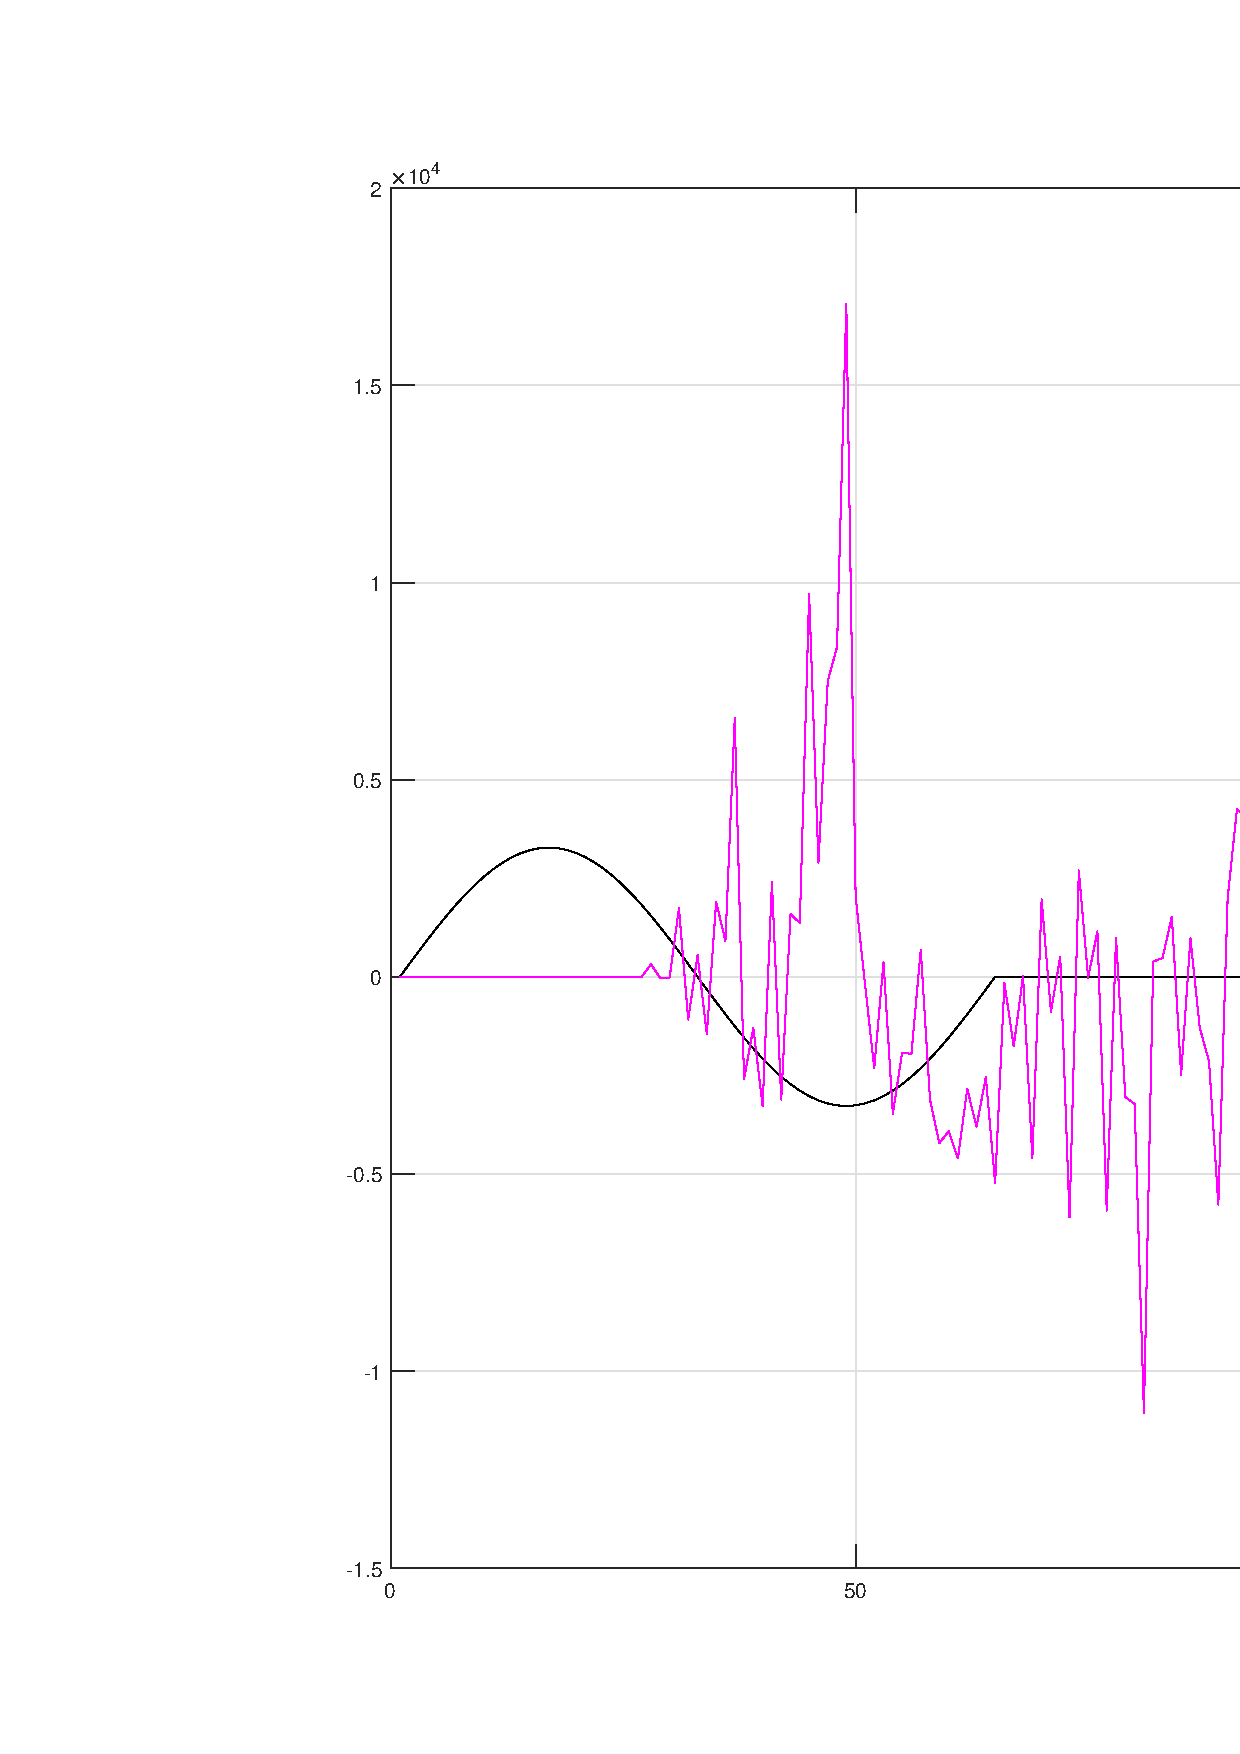
\includegraphics{../../buch/chapters/7-algo/images/db4.pdf}
\end{center}
\end{frame}


